\section{Modelado experimental y resultados}
\label{sec:modelado-resultados}

La actividad técnica añade un prototipo local reproducible en \texttt{notebooks/04\_implementacion\_tecnica\_3\_1\_2.ipynb}. Se entrena sobre los 302 registros únicos, con partición estratificada de 226 observaciones para entrenamiento y 76 para prueba (semilla 42). Los modelos nuevos utilizan codificación one-hot para predictores categóricos; la regresión logística aplica \texttt{RobustScaler} a variables cuantitativas. El preprocesamiento se ajusta dentro del pipeline de validación cruzada para evitar fuga de información.

Se compararon cinco folds sobre el conjunto de entrenamiento. La regresión logística de referencia obtuvo ROC-AUC medio de 0,919 $\pm$ 0,052; XGBoost one-hot somero obtuvo 0,914 $\pm$ 0,055; XGBoost one-hot regularizado 0,913 $\pm$ 0,061; y el baseline XGBoost ordinal 0,917 $\pm$ 0,062. Se eligió el XGBoost one-hot somero como artefacto final para cumplir el requisito de entrenamiento local con GPU, aunque no tuvo el mayor promedio de validación cruzada.

En la prueba retenida, el baseline ordinal obtuvo accuracy 0,789, precisión de clase positiva 0,791, recall 0,829, F1 0,810 y ROC-AUC 0,875. El XGBoost one-hot seleccionado obtuvo 0,776, 0,786, 0,805, 0,795 y 0,875, respectivamente. Así, la nueva representación trata las variables categóricas de manera más adecuada, pero no mejoró las métricas predictivas de esta partición; ambas versiones empataron en ROC-AUC. Con sólo 76 casos de prueba no se afirma diferencia estadística ni superioridad predictiva.

\begin{figure}[H]
  \centering
  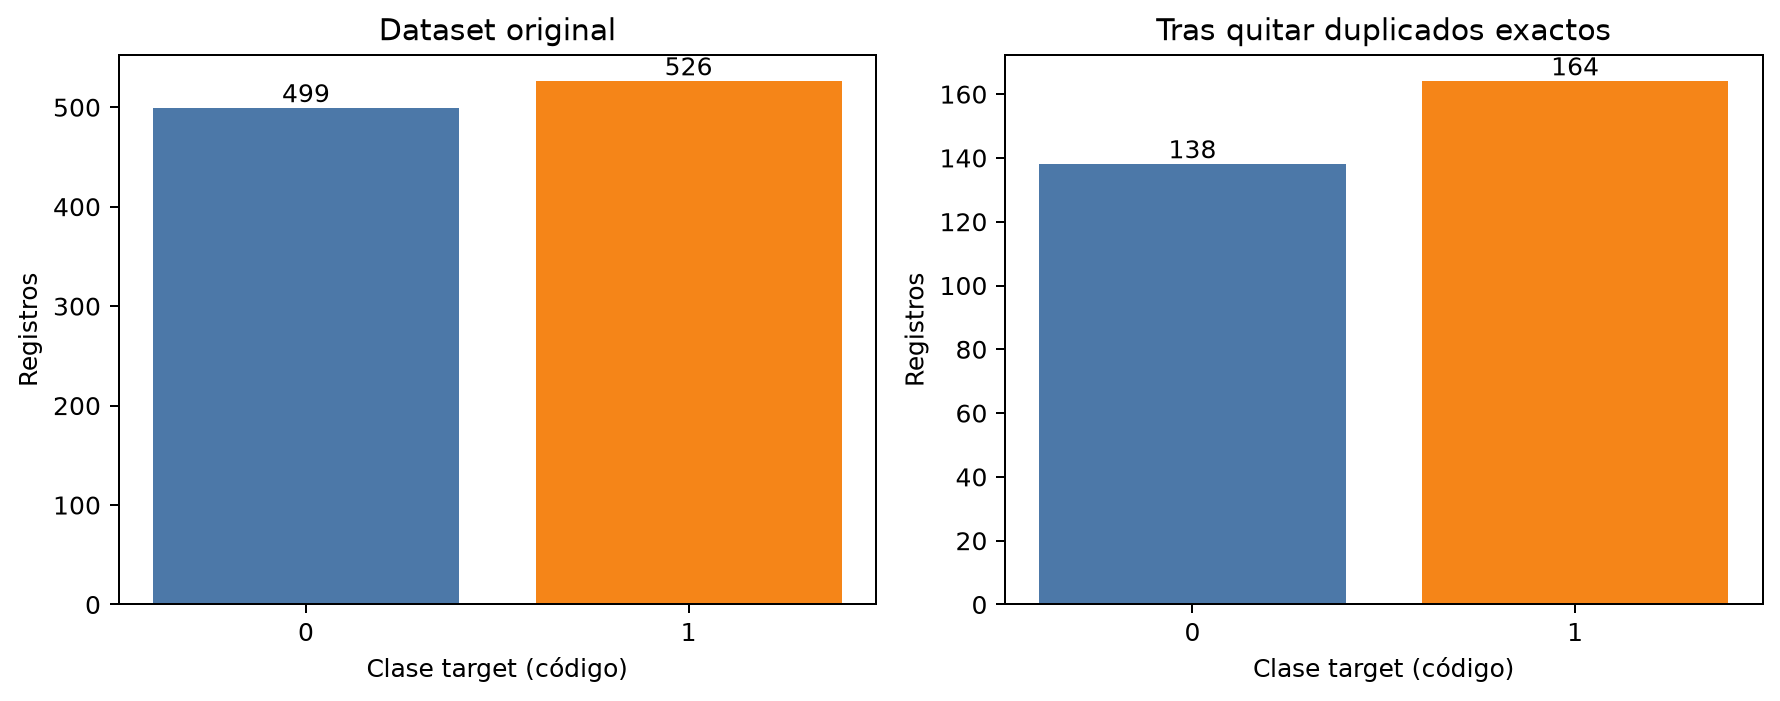
\includegraphics[width=0.88\textwidth]{../outputs/figures/distribucion_clases_antes_despues_deduplicar.png}
  \caption{Distribución de clases antes y después de deduplicar. El cambio de proporciones respalda documentar el tratamiento de duplicados antes de particionar.}
  \label{fig:clases-deduplicacion}
\end{figure}

\begin{figure}[H]
  \centering
  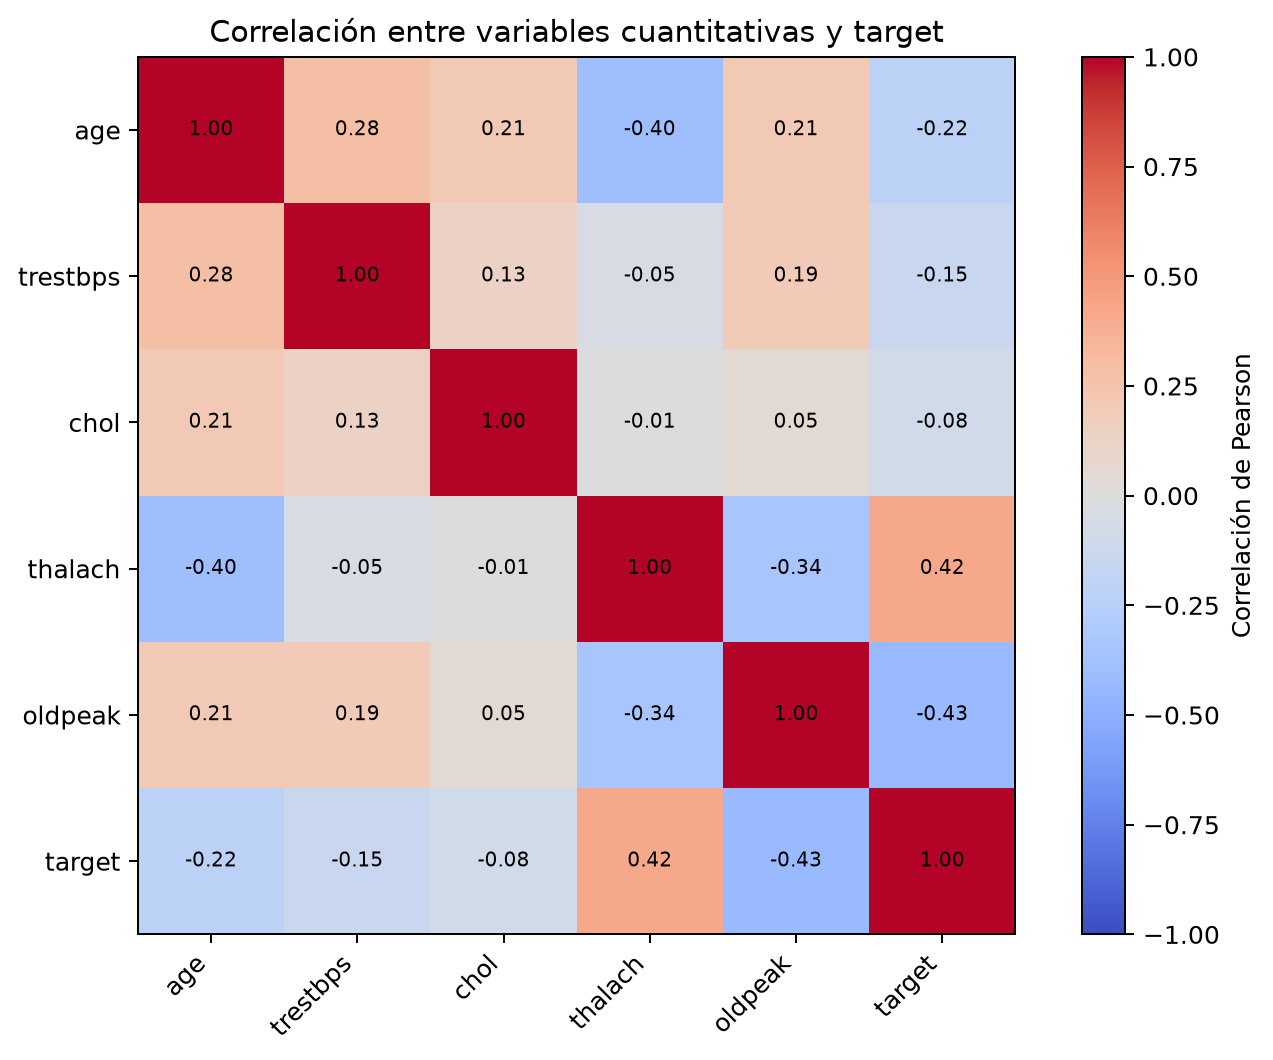
\includegraphics[width=0.9\textwidth]{../outputs/figures/matriz_correlacion_continuas_target.png}
  \caption{Correlación Pearson de variables cuantitativas con \texttt{target}. Es una asociación descriptiva, no evidencia causal.}
  \label{fig:correlacion-modelado}
\end{figure}

\begin{figure}[H]
  \centering
  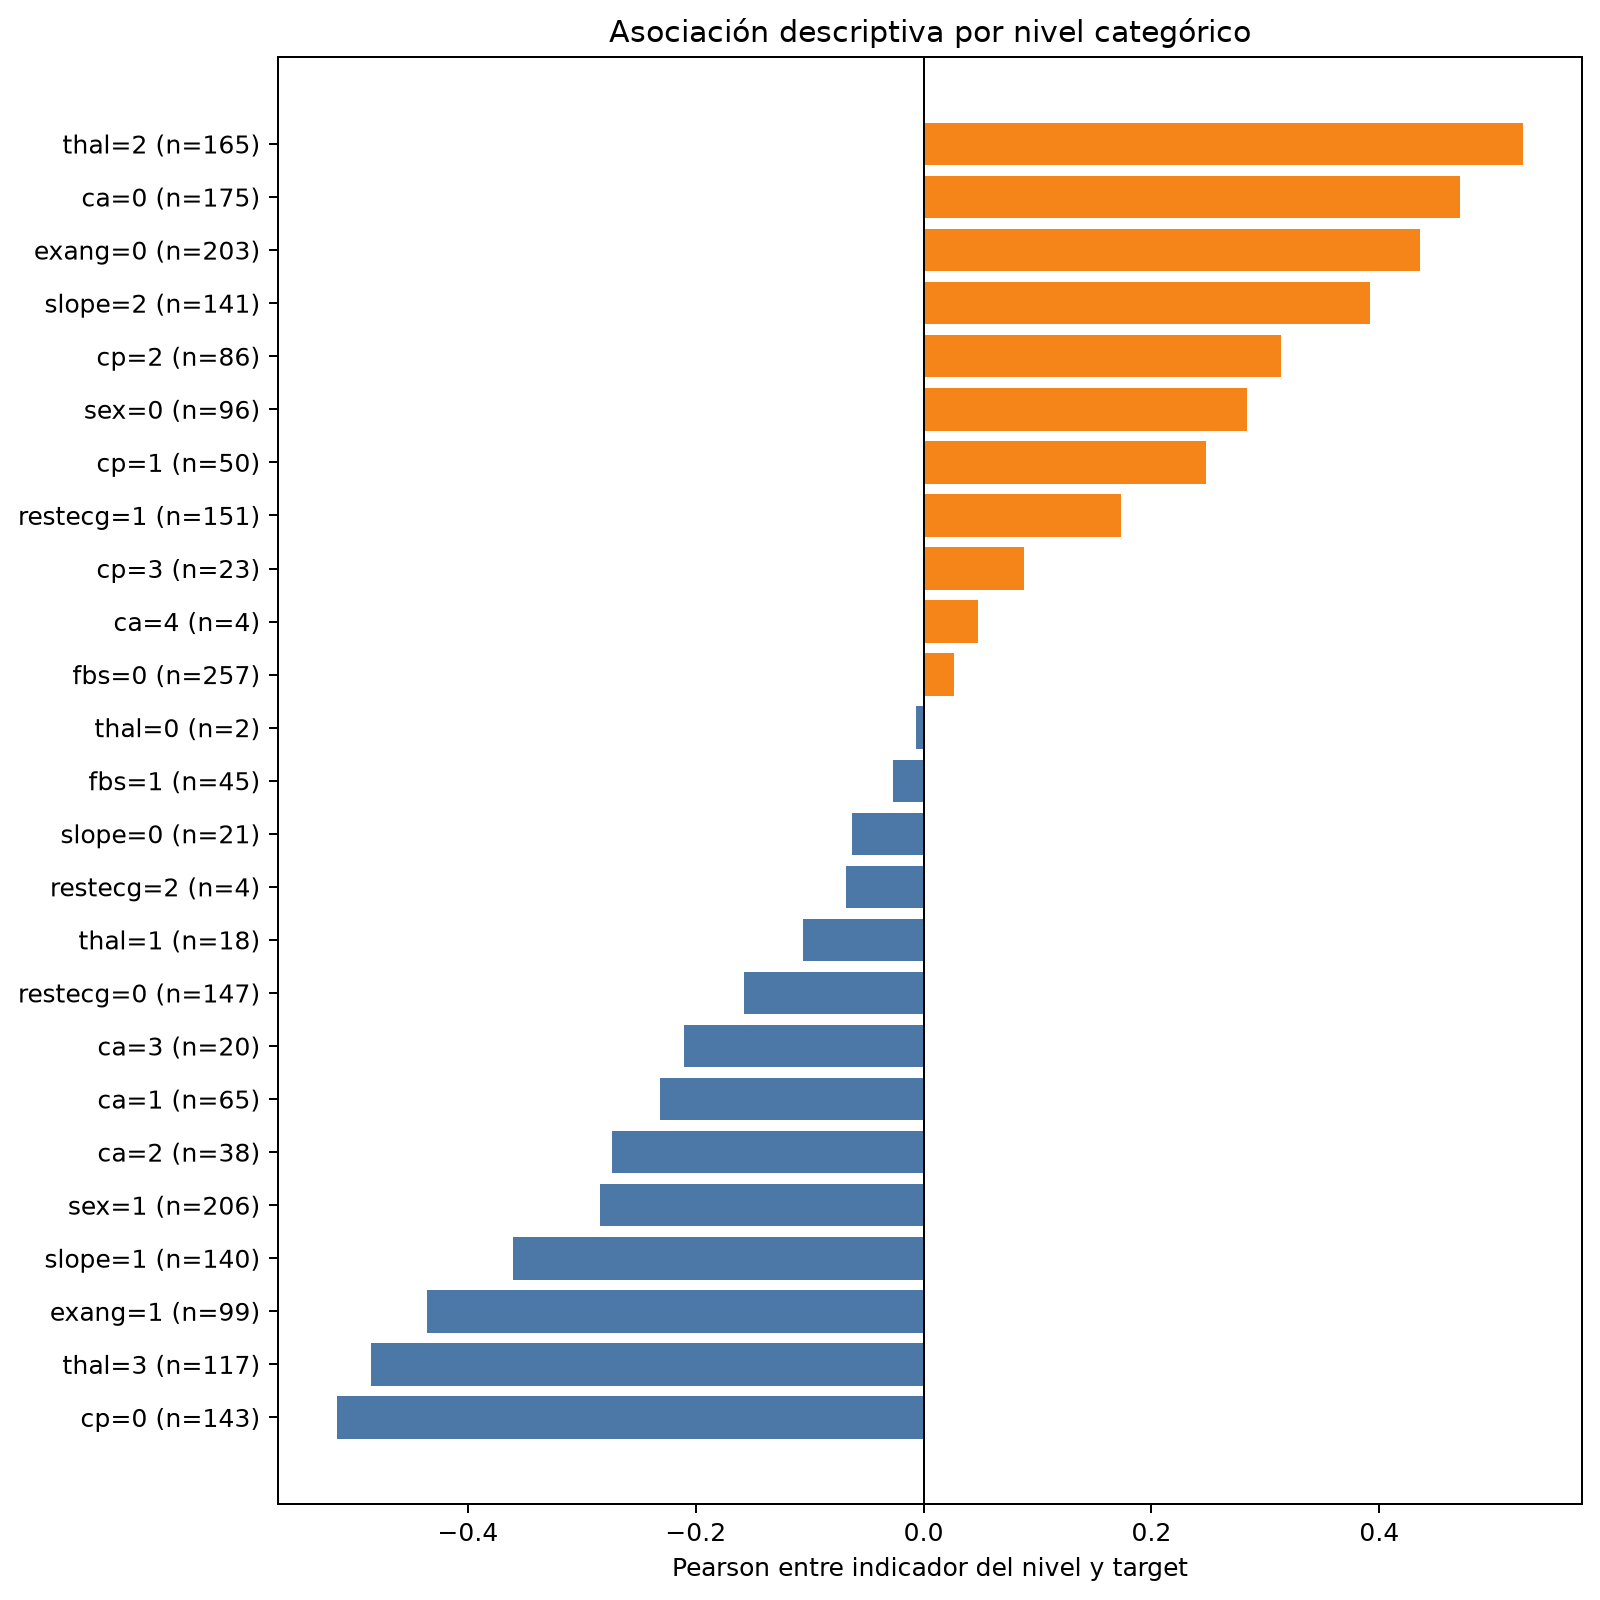
\includegraphics[width=0.9\textwidth]{../outputs/figures/asociacion_niveles_categoricos_target.png}
  \caption{Asociación descriptiva entre niveles categóricos y \texttt{target}; los tamaños de muestra varían entre niveles.}
  \label{fig:asociacion-categorica}
\end{figure}

\begin{figure}[H]
  \centering
  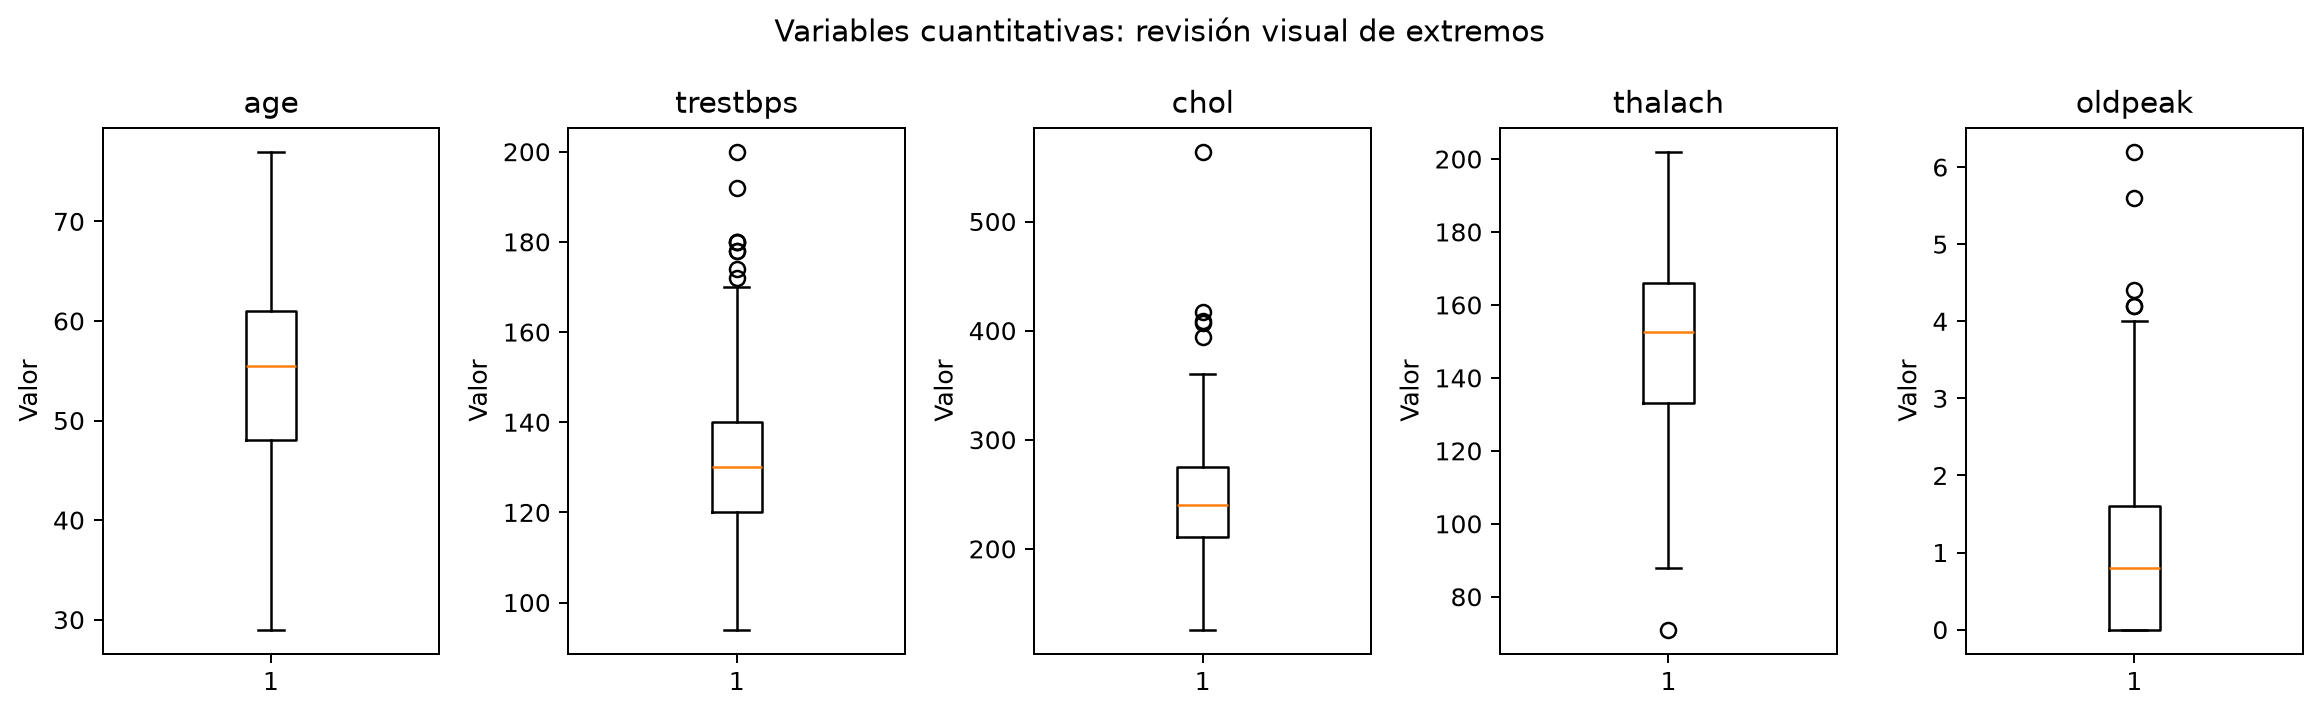
\includegraphics[width=0.9\textwidth]{../outputs/figures/diagramas_caja_variables_cuantitativas.png}
  \caption{Distribuciones y valores candidatos a revisión por la regla de 1,5 IQR. Los extremos se conservaron porque no se confirmaron como errores.}
  \label{fig:outliers-modelado}
\end{figure}

\begin{figure}[H]
  \centering
  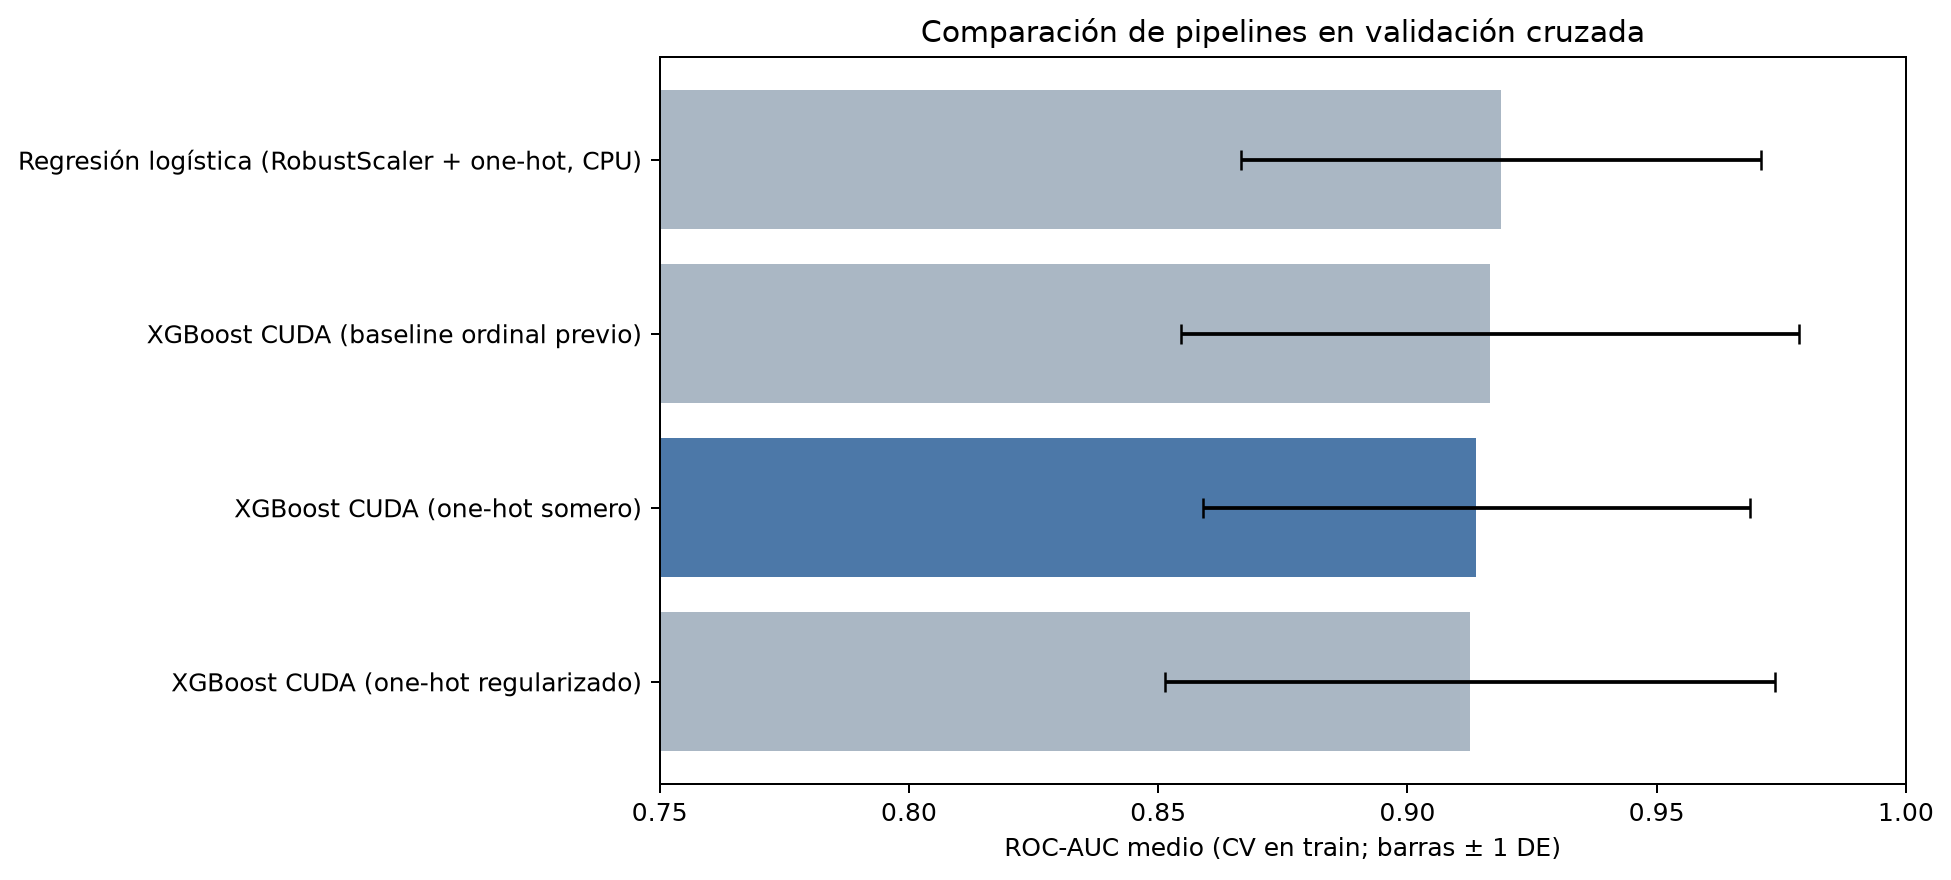
\includegraphics[width=0.88\textwidth]{../outputs/figures/comparacion_roc_auc_validacion_cruzada.png}
  \caption{ROC-AUC medio y dispersión en validación cruzada para pipelines evaluados sobre los mismos folds.}
  \label{fig:roc-cv}
\end{figure}

\begin{figure}[H]
  \centering
  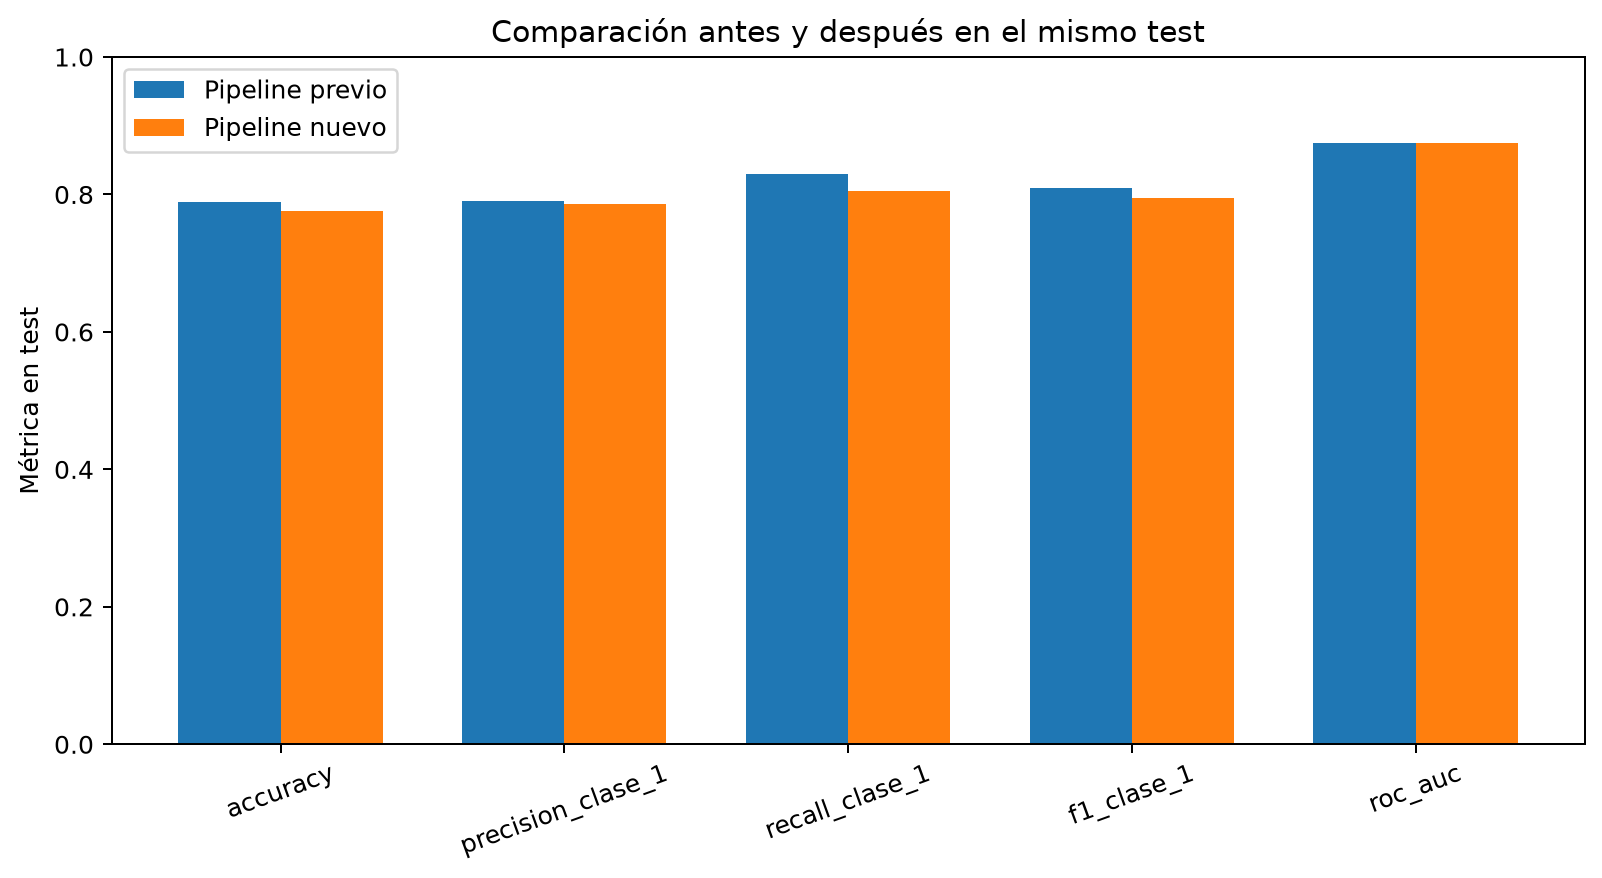
\includegraphics[width=0.9\textwidth]{../outputs/figures/comparacion_metricas_test_antes_despues.png}
  \caption{Métricas del baseline ordinal y del modelo one-hot en la misma partición de prueba. No se observa mejora general del modelo nuevo.}
  \label{fig:metricas-test-modelos}
\end{figure}

El artefacto \texttt{outputs/models/heart\_disease\_pipeline.joblib} registra entrenamiento con XGBoost 3.2.0 y \texttt{cuda:0} en una NVIDIA GeForce RTX 4060 Laptop GPU. La automatización \texttt{src/automatizacion\_predicciones.py} procesa cinco filas sintéticas de ejemplo; sus scores no están calibrados y no son probabilidades clínicas. El modelo no está desplegado, no se evaluó en datos locales chilenos y no se autoriza para diagnóstico, tratamiento o priorización asistencial.

Los gráficos, tablas, entorno \texttt{uv} y pasos de ejecución se describen en \texttt{docs/implementacion\_tecnica\_3\_1\_2.md}. La guía solicita además guardar el notebook en Google Drive; este repositorio sólo acredita la copia local, por lo que no afirma que ese requisito externo se haya completado.
